\begin{wrapfigure}[8]{r}{0.25\textwidth}
\vspace{-1.0em}\centering\strut
%\includegraphics[width=0.4\textwidth,clip,trim=1cm 2.5cm 1cm 1cm]{figs/teasers/teaser-computation-v2.pdf}
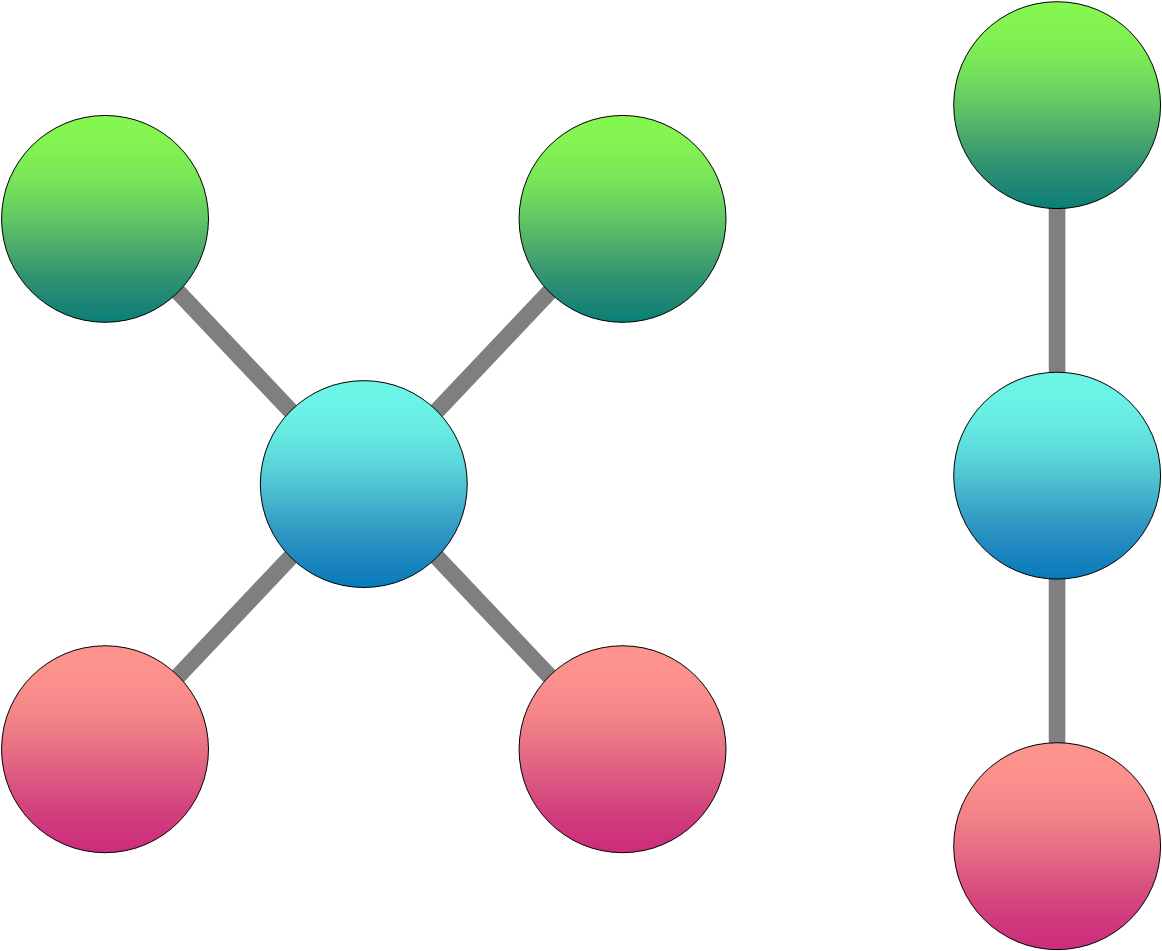
\includegraphics[width=0.2\textwidth]{figure/attention_not_distinguish.png}
\vspace{-0.5em}
\caption{\textbf{Examples of graphs hard for pure attention to distinguish.}}
\label{fig:attention_not_distinguish}
\end{wrapfigure}

\subsection{Edge-Degree Embedding}
\label{subsec:edge_degree_embedding}


Softmax in equivariant graph attention calculates weighted averages over all neighboring nodes.
Therefore, there exist some cases where attention cannot distinguish between two different graphs.
For example, the two graphs in Fig.~\ref{fig:attention_not_distinguish} cannot be distinguished by attention if we only consider scalars and features on nodes of the same colors are identical.
This results in the same output of attention for two different graphs.

Degree information is indispensable to differentiate between the two graphs, and therefore, we propose edge-degree embedding to address the issue.
As depicted in the right branch in  Fig.~\ref{fig:equiformer}(c), we first transform a constant one vector into messages encoding local geometry with two linear layer and one intermediate DTP layer.
The DTP layer has the same form as that in Eq.~\ref{eq:pre_attn}.
We then use sum aggregation~\cite{gin} to encode degree information.
We scale the aggregated features by dividing with the squared root of average degrees in training sets so that standard deviation of aggregated features would be close to $1$.
Including degree information can easily differentiate the two graphs, and therefore, we place edge-degree embedding at the beginning of Equiformer.